% LTex: language=pl
\section{Opis systemu STOS}
\indent System Testowania i~Oceny zadań Studenckich (w skrócie „STOS”), to system dedykowany dla prowadzących zajęcia na Politechnice Gdańskiej. Umożliwia testowanie rozwiązań stworzonych przez studentów podczas zajęć projektowych oraz laboratoryjnych, pod kątem wydajności i~poprawności. Przepływ pracy polega na przesłaniu kodu programu przez studenta do systemu, kompilacji po stronie serwera oraz przesłaniu wyniku na podstawie serii testów zdefiniowanych przez prowadzącego.

\section{Komponenty i~schemat działania}
System możemy podzielić na komponenty ze względu na realizowane zadania:
\begin{itemize}
    \item STOS -- serwis w~postaci strony internetowej, umożliwiający wgranie rozwiązań przez studentów i~umieszczenie ich w~kolejce dostępnej do pobrania przez inne serwisy poprzez żądania HTTP.
    \item Moduł sprawdzający -- część serwisu działającego po stronie serwera. Jego zadaniem, jest wywoływanie zapytań do API STOS-u metodą odpytywania, w~celu pobierania kodu programów do wykonania, zlecenie kompilacji, ocenę kodu oraz przesłanie wyniku do STOS-u.
    \item Moduł kompilujący -- skonteneryzowany serwis działający na serwerze, kompilujący otrzymany kod. Ma możliwość kompilacji lub interpretacji wielu języków programowania. Aktywnie nasłuchuje komunikatów przesyłanych przez nazwany potok. Jest przystosowany do ciągłego działania, co wymaga uruchomienia go wyłącznie przy starcie całej platformy. Posiada współdzielone katalogi z~gospodarzem, zawierające skrypty kontrolujące, kody źródłowe oraz rezultaty.
\end{itemize}
\begin{figure}
	\begin{center}
		\resizebox{1.0\textwidth}{!} {
			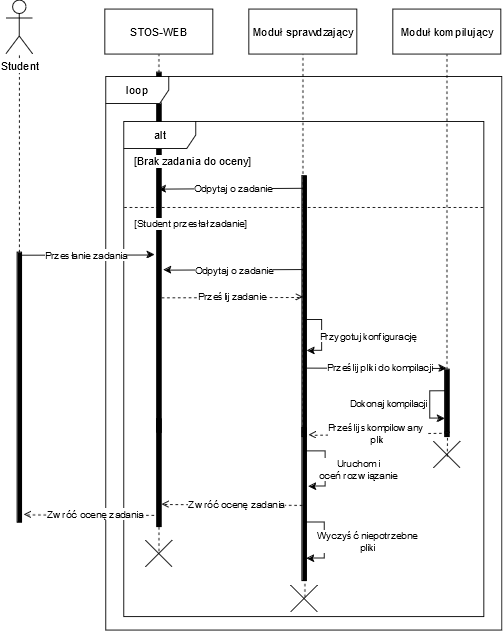
\includegraphics{img/1/d_sek_1.png}
		}
		\caption[Diagram sekwencji komponentów]{Diagram przedstawiający sekwencję wykonywanych zdarzeń w~systemie, podczas oceny zadania. Źródło własne.}
	\end{center}
\end{figure}
